\section{Orthogonal Polynomials in \texorpdfstring{$(-1,1)$}{(-1,1)}}

\subsection{Sturm-Liouville problem}

The solution of many differential equations relies on solving problems of the following type
\begin{equation}
    \tag{SL}
    \label{eq:Sturm-Liouville}
    \begin{dcases}
        -\frac{d}{dx}\left(p\frac{du}{dx}\right) + q u = \lambda w u & \text{in } (-1,1) \\
        \text{suitable boundary conditions}
    \end{dcases}
\end{equation}
Here
$p$ is continuously differentiable, strictly positive in $(-1, 1)$ and continuous at $x = \pm 1$; $q$ is continuous, nonnegative and bounded in $(-1, 1)$; the weight function $w$ is continuous, nonnegative and integrable over $(-1, 1)$. $\lambda$ is usually known.

\subsection{Orthogonal systems of polynomials}
Given $w: (-1,1) \to \mathbb R$ we define
\begin{equation*}
    (u,v)_w = \int_{-1}^1 u(x)v(x)w(x)dx.
\end{equation*}
Using Gram-Schmidt we can find $L^2_w(-1,1)$-orthogonal polynomials $p_k$ such that $\degree p_k = k$.
Similarly to Fourier series we can define
\begin{equation*}
    \hat u_k = \frac{1}{\|p_k\|_w^2} \int_{-1}^1 u(x) p_k(x) w(x) dx.
\end{equation*}
And we have the finite projection
\begin{equation*}
    P_N u = \sum_{k=0}^N \widehat u_k p_k.
\end{equation*}
Notice that we have the characterisation via the inner product
\begin{equation*}
    (P_N u , v)_w = (u,v)_w, \qquad \forall v \in \mathbb R_N[x].
\end{equation*}
Weierstrass' theorem implies that this system is complete in $L^2_w(-1,1)$, i.e.
\begin{equation*}
    \lim_{N\to\infty}\|u - P_N u\|_{w} \to 0
\end{equation*}

\begin{remark}[Sturm-Liouville problems with $p(\pm 1) = 0$]
    \label{rem:Sturm-Liouville degenerate}
    When $p(\pm 1) = 0$ the Sturm-Liouville operator is self-adjoint without imposing any boundary conditions. Notice that if $u,v \in C^1([a,b])$ then
    \begin{align*}
        -\int_{-1}^1\frac{d}{dx}\left(p\frac{du}{dx}\right)v
         & = -\int_{-1}^1\frac{d}{dx}\left(p\frac{du}{dx}v \right) + \int_{-1}^1p\frac{du}{dx} \frac{dv}{dx}
        \\
         & = - p \frac{du}{dx} v\Big|_{-1}^1 + \int_{-1}^1 p\frac{du}{dx}  \frac{dv}{dx}
        \\
         & =  \int_{-1}^1 p\frac{du}{dx}\frac{dv}{dx}
    \end{align*}
    We can integrate by parts again.
    Then, if $u_\lambda, u_\mu \in C^1([a,b])$ are such that
    \begin{equation*}
        -\frac{d}{dx}\left(p\frac{du_\lambda}{dx}\right) + q u_\lambda = \lambda w u_\lambda \text{ in } (-1,1), \qquad -\frac{d}{dx}\left(p\frac{du_\mu}{dx}\right) + q u_\mu = \mu w u_\mu  \text{ in } (-1,1)
    \end{equation*}
    of different eigenvalues are $L^2_w$ orthogonal
    \begin{align*}
        \lambda \int_{-1}^1 u_\lambda u_\mu w
         & = -\int_{-1}^1 \frac{d}{dx} \left( p \frac{du_\lambda}{dx} \right) u_\mu + \int_{-1}^1 q u_\lambda u_\mu
        \\
         & = -\int_{-1}^1 u_\mu \frac{d}{dx} \left( p \frac{du_\mu}{dx} \right) + \int_{-1}^1 q u_\lambda u_\mu     \\
         & = \mu \int_{-1}^1 u_\lambda u_\mu w.
    \end{align*}
    If $\mu \ne \mu$ then $(u_\lambda, u_\mu)_w = 0$.
\end{remark}

\subsection{Polynomial interpolation}

On the other hand, let us define for a given choice of nodes $x_0, \cdots, x_{N+1}$ the interpolation polynomial by
\begin{equation*}
    I_N : C([-1,1]) \to \mathbb R_N[x], \qquad \text{ such that } I_N u(x_j) = u(x_j).
\end{equation*}
We will not make the dependence of $I_N$ on the set of nodes explicit. This should not lead to confusion.
\begin{remark}
    Notice that if $u^N \in \mathbb R_N$ then $I_N u^N = u^N$, independently of the basis of points chosen.
\end{remark}
We define the Lebesgue constant
\begin{equation*}
    \Lambda_N = \sup_{v \in C([-1,1])} \frac{\| I_N v \|_{L^\infty(-1,1)}}{\| v \|_{L^\infty(-1,1)}}.
\end{equation*}
It can be expressed as function of the Lagrange polynomials based on the same points
\begin{equation*}
    \Lambda_N = \max_{x \in [-1,1]} \sum_{j=0}^N |L_j(x)|.
\end{equation*}

\paragraph{Interpolation error}
We recall the formula \eqref{eq:Lagrange interpolation error estimate} for the interpolation error. It says that
\begin{equation*}
    \| u - I_N u \|_{L^\infty(-1,1)} \le [u]_{W^{N+1,\infty}} \frac 1 {(N+1)!} \max_{x \in [-1,1]} \prod_{k=0}^N |x-x_k|.
\end{equation*}

If we use $N+1$ equi-distant points $x_k$ we get
\begin{equation*}
    \| u - I_N u \|_{L^\infty(-1,1)} \le \frac{2^{N-1}}{N+1} [u]_{W^{N+1,\infty}(-1,1)}
\end{equation*}
If we choose the interpolation more wisely, we get much better rates of convergence
\begin{theorem}
    Given the we use the Chebyshev nodes $x_k = \cos \frac{(2k+1) \pi}{2N+2}$ for $k=0, \cdots, N$ we can estimate
    \begin{equation}
        \label{eq:interpolation error Chebyshev nodes}
        \| u - I_N u \|_{L^\infty(-1,1)} \le \frac{1}{2^N (N+1)!} [u]_{W^{N+1,\infty}(-1,1)}
    \end{equation}
\end{theorem}
\begin{proof}
    The Chebyshev nodes are the roots of the Chebyshev polynomial of the first kind $T_N$ presented in \Cref{sec:Chebyshev polynomials}.
    Since they both have $N+1$ different roots and of degree $N+1$, we have that $\prod_{k=0}^N (x-x_k) = c_N T_{N}(x)$ up to a constant $c_N \in \mathbb R$.
    The polynomial $\prod_{k=0}^N (x-x_k)$ has leading coefficient $1$, whereas the leading coefficient of $T_N$ is $2^N$ (see \Cref{eq:Chebyshev recursion}). Therefore, $c_N = 2^{-N}$. Due to \eqref{eq:Chebyshev Tn} we have that $\|T_N\|_{L^\infty(-1,1)} = 1$.
\end{proof}



\paragraph{Runge's phenomenom}
\label{sec:Runge's phenomenon}

Polynomial interpolation of a function in an interval can lead to oscillations (see \Cref{fig:Runge})
even though we have the formula \eqref{eq:Lagrange interpolation error estimate} for the interpolation error.
The classical example is equi-distintant points $x_k$ in $[-1,1]$ and Runge's function $f(x) = \frac{1}{1+25x^2}$.
The reason is two-fold
\begin{enumerate}
    \item For Runge's function  $\frac{d^n f}{dx^n}$ grows rapidly with $n$.

    \item The fact that the points are equi-distant makes the error constant not decay fast enough.
\end{enumerate}
The interpolation may not converge uniformly if the interpolation points are not well-chosen.
\begin{figure}[H]
    \centering
    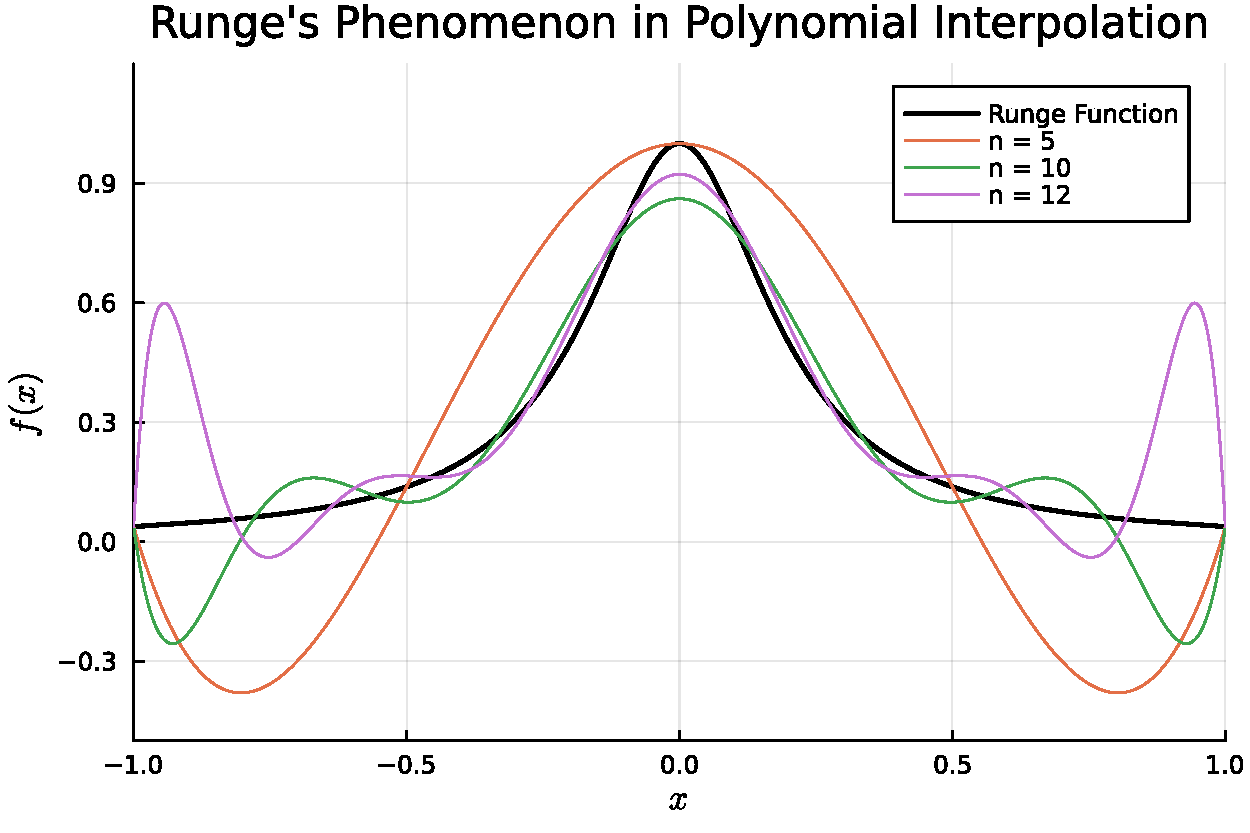
\includegraphics[width=0.5\textwidth]{Runge}
    \caption{Runge's phenomenon for $I_n u$ using uniformly distributed nodes $x_j$, where each $I_n$ intersects the Runge function $f(x) = \frac{1}{1+25x^2}$.
    }
    \label{fig:Runge}
\end{figure}
This effect is specially noticeable near the boundary if we use uniformly positioned weights. This is way interpolation with ``smartly chosen points is interesting''. To mitigate this effect, some authors use singular weights on the boundary like $w(x) = (1-x^2)^{-\frac 1 2}$.

\subsection{Gauss-type quadrature and polynomial transform}

The standard Gaussian quadrature
\begin{strongtheorem}[Gauss' quadrature]
    \label{thm:Gauss integration}
    Let $p_k$ be orthogonal in $L^2_w$ with $\degree p_k = k$, $x_0, \cdots, x_N$ be the roots of $p_{N+1}$, and let $w_0, \cdots, w_N$ be the solutions to
    \begin{equation*}
        \sum_{j=0}^N (x_j)^k w_j = \int_{-1}^1 x^k w(x) dx, \qquad 0 \le k \le N.
    \end{equation*}
    Then $w_j > 0$ and we have integration formula
    \begin{equation}
        \label{eq:Gauss integration}
        \sum_{j=0}^N p(x_j) w_j = \int_{-1}^1 p(x) w(x) dx \qquad \forall p \in \mathbb R_{2N+1}[x].
    \end{equation}
    Furthermore, there are no weights such that equality holds in $\mathbb R_{2N+2}[x]$.
\end{strongtheorem}
In some applications, for example to solve boundary-value problems, it is preferable that the end-points of the interval evaluation points. This rules are called \emph{Gauss-Lobatto} quadrature rules.
\begin{strongtheorem}[Gauss-Lobatto integration with Jacobi weights]
    \label{thm:Gauss-Lobatto integration Jacobi weights}
    Let $w_{\alpha,\beta}(x) = (x - 1)^\alpha (1 + x)^\beta$ with $\alpha, \beta > -1$.
    Let $J^{(\alpha,\beta)}_k$ denote the $k$-th Jacobi polynomial (i.e., the orthogonal basis of $L^2_w(-1,1)$ with $\deg J^{(\alpha,\beta)}_k=k$).
    Let
    \begin{equation*}
        x_0 = -1, x_N = 1, \qquad, x_1, \cdots, x_{N-1} \text{ be the zeros of } \frac{dJ_N^{(\alpha,\beta)}}{dx}.
    \end{equation*}
    and
    let $w_0, \cdots, w_N$ be the solutions to
    \begin{equation*}
        \sum_{j=0}^N (x_j)^k w_j = \int_{-1}^1 x^k w(x) dx, \qquad 0 \le k \le N.
    \end{equation*}
    Then we have that
    \begin{equation}
        \label{eq:Gauss-Lobatto integration}
        \sum_{j=0}^N p(x_j) w_j = \int_{-1}^1 p(x) w(x) dx \qquad \forall p \in \mathbb R_{2N-1}[x].
    \end{equation}
\end{strongtheorem}
For a proof see \cite{QuarteroniSaccoSaleri2007}.

\subsection{Differentiation}

Let us define
\begin{equation*}
    \mathcal D_N u = \frac{d I_N u}{dx}
\end{equation*}
For collocation methods we usually
we will use the matrices
\begin{equation*}
    \begin{pmatrix}
        \frac{d I_N u}{dx} (x_1) \\
        \vdots                   \\
        \frac{d I_N u}{dx} (x_{N-1})
    \end{pmatrix}
    =
    \mat D_N
    \begin{pmatrix}
        u(x_0)      \\
        u (x_1)     \\
        \vdots      \\
        u (x_{N-1}) \\
        u(x_N)
    \end{pmatrix},
    \qquad
    \begin{pmatrix}
        \frac{d^2 I_N u}{dx^2} (x_1) \\
        \vdots                       \\
        \frac{d^2 I_N u}{dx^2} (x_{N-1})
    \end{pmatrix}
    =
    \mat D^{(2)}_N
    \begin{pmatrix}
        u(x_0)      \\
        u (x_1)     \\
        \vdots      \\
        u (x_{N-1}) \\
        u(x_N)
    \end{pmatrix}
\end{equation*}

\begin{example}[Collocation method in matrix form]
    Let $x_0 < x_1 < \cdots < x_N$ and assume we want to solve
    the collocation method: find $u^N \in \mathbb R_N[x]$ such that
    \begin{equation*}
        \begin{dcases}
            -\frac{d^2 u^N }{dx^2} (x_j) = f(x_j) & \text{for } j \in \{1, \cdots, N-1\} \\
            u^N(x_0) = g(x_0),                                                           \\
            u^N (x_N) = g(x_N)
        \end{dcases}
    \end{equation*}
    Since $u^N \in \mathbb R_N[x]$ we have that $I_N u^N = u^N$.
    Using this matrices we can write the system using block matrices as
    \begin{equation*}
        \begin{pmatrix}
            1                      \\
             & -\mat D_N^{(2)}     \\
             &                 & 1
        \end{pmatrix}
        \begin{pmatrix}
            u(x_0)      \\
            u (x_1)     \\
            \vdots      \\
            u (x_{N-1}) \\
            u(x_N)
        \end{pmatrix}
        = \begin{pmatrix}
            g(x_0)      \\
            f (x_1)     \\
            \vdots      \\
            f (x_{N-1}) \\
            g(x_N)
        \end{pmatrix}
    \end{equation*}
\end{example}